
%%%%%%%%%%%%%%%%%%%%%%%%%%%%%%%%%%%%%%%%%%%%%%%%%%%%%%%%%
% Niniejszy plik przedstawia przykładowy skład 
% pracy dyplomowej na Wydziale Matematyki PWr. 
% 
% Autorzy: 
% Damian Fafuła
% Michał Kijaczko
% Jakub Michalczak
% Maciej Miśta
% Dagmara Nowak
% Tomasz Skalski
% Wojciech Słomian
%
%% Data utworzenia: 8.05.2018
% Numer wersji: 1
%
% Poniższą formatkę można rozpowszechniać i edytować 
% pod warunkiem zachowania numeru wersji, 
% informacji o autorach i dodaniu informacji 
% o wprowadzonych zmianach.
%
%%%%%%%%%%%%%%%%%%%%%%%%%%%%%%%%%%%%%%%%%%%%%%%%%%%%%%%%%
% Domyślną opcją jest: praca magisterska, język polski.
% W przypadku pracy pisanej w języku angielskim dodajemy 
% opcję [english].
% Dla pracy licencjackiej dodajemy opcję [licencjacka].
% Dla pracy inżynierskiej dodajemy opcję [inzynierska].
% Dopuszczalne są podwójne opcje, np. [licencjacka, english].
% Opcje dodajemy w kwadratowym nawiasie przy \documentclass.
%
%
%%%%%%%%%%%%%%%%%%%%%%%%%%%%%%%%%%%%%%%%%%%%%%%%%%%%%%%%%
\documentclass[inzynierska]{pwr_wmat_praca_dyplomowa}

%%%%%%%%%%%%%%%%%%%%%%%%%%%%%%%%%%%%%%%%%%%%%%%%%%%%%%%%%
%              DANE DO PRACY
%
% W przypadku pracy dyplomowej w języku angielskim nie jest konieczne 
% wypełnianie pól: \tytul{}, \kierunek{}, \specjalnosc{}, 
%                  \streszczenie{}, \slowakluczowe{}.
%%%%%%%%%%%%%%%%%%%%%%%%%%%%%%%%%%%%%%%%%%%%%%%%%%%%%%%%%
%
% Imię i nazwisko autora
\autor{Paweł Budzyński}
%
% Tytuł pracy dyplomowej 
\tytul{Wykorzystanie sieci neuronowych w problemie wykrywania uszkodzeń lokalnych w maszynach górniczych} 
\tytulang{The neural networks in the problem of local damage detection in mining machines}
%
% Tytuł / stopień / imię i nazwisko opiekuna
\opiekun{dr hab. inż. Agnieszka Wyłomańska}
%
% Kierunek studiów wybieramy spośród następujących:
% 1) Matematyka
% 2) Matematyka i Statystyka
% 3) Matematyka stosowana
\kierunekstudiow{Matematyka Stosowana}
%
% Kierunek studiów po angielsku wybieramy spośród następujących:
% 1) Mathematics
% 2) Mathematics and Statistics
% 3) Applied Mathematics
\kierunekstudiowang{Applied Mathematics}
%
% Specjalność wybieramy spośród następujących: 
% KIERUNEK: Matematyka
% 1) Matematyka teoretyczna,
% 2) Statystyka matematyczna,
% 3) Matematyka finansowa i ubezpieczeniowa,
%
% KIERUNEK: Matematyka i Statystyka
% 4) Matematyka,
% 5) Statystyka i analiza danych, 
%
% 6) -- (w przypadku braku specjalizacji).
\specjalnosc{--} 
%
% Specjalność w języku angielskim wybieramy spośród następujących:
% KIERUNEK: Matematyka
% 1) Theoretical Mathematics,
% 2) Mathematical Statistics,
% 3) Financial and Actuarial Mathematics,
%
% KIERUNEK: Matematyka i Statystyka
% 4) Mathematics,
% 5) Statistics and Data Analysis,
%
% KIERUNEK: Applied Mathematics
% 6) Financial and Actuarial Mathematics, 
% 7) Mathematics for Industry and Commerce,
% 8) Computational Mathematics,
% 9) Modelling, Simulation and Optimization.
%
% 10) -- (w przypadku braku specjalizacji).
\specjalnoscang{--} 
%
% Krótkie streszczenia po polsku i angielsku
% - nie dłuższe niż 530 znaków.
\streszczenie{Celem pracy jest zastosowanie sieci neuronowych do analizy sygnałów drganiowych w celu wykrywania uszkodzeń lokalnych w maszynach górniczych. Zakres pracy obejmuje opracowanie nowych metod i ich zastosowanie}
\streszczenieang{sieci neuronowe, nauczanie maszynowe, szeregi czasowe,}
%
% Podajemy najważniejsze słowa kluczowe po polsku i angielsku
% - w obu przypadkach, nie więcej niż 150 znaków.
\slowakluczowe{tutaj podajemy najważniejsze słowa kluczowe (łącznie nie powinny być dłuższe niż 150 znaków).}  
\slowakluczoweang{tutaj podajemy najważniejsze słowa kluczowe w języku angielskim (łącznie nie powinny być dłuższe niż 150 znaków)}
%
%
%%%%%%%%%%%%%%%%%%%%%%%%%%%%%%%%%%%%%%%%%%%%%%%%%%%%%%%%%
% Definicje, lematy, twierdzenia, przykłady i wnioski
% Komendy wywołujące twierdzenia, definicje, itd., 
% czyli 'theorem', 'definition', 'corollary', itd., 
% można zmienić wedle uznania.
\theoremstyle{plain}
\newtheorem{theorem}{Twierdzenie}
\numberwithin{theorem}{chapter}
\newtheorem{lemma}[theorem]{Lemat} 
\newtheorem{corollary}[theorem]{Wniosek}
\newtheorem{fact}[theorem]{Fakt}
\theoremstyle{definition}
\numberwithin{theorem}{chapter}
\newtheorem{definition}[theorem]{Definicja} 
\newtheorem{example}[theorem]{Przykład}
\newtheorem{note}[theorem]{Uwaga}
%%%%%%%%%%%%%%%%%%%%%%%%%%%%%%%%%%%%%%%%%%%%%%%%%%%%%%%%%
\usepackage{cite}

%%%%%%%%%%%%%%%%%%%%%%%%%%%%%%%%%%%%%%%%%%%%%%%%%%%%%%%%%
%%%%%%%%%%%%%%%%%%%%%%%%%%%%%%%%%%%%%%%%%%%%%%%%%%%%%%%%%
\begin{document}
\frontmatter
\maketitle
\mainmatter
\tableofcontents
%\listoffigures
%\listoftables



{\backmatter \chapter{Wstęp}}

%\chapter{Uszkodzenia lokalne oraz ich wykrywanie}
Tematem pracy jest wykorzystanie sieci neuronowych w problemie wykrywania uszkodzeń lokalnych w maszynach górniczych. Zadanie polega na przetworzeniu sygnału diagnostycznego oraz dokonaniu na jego podstawie decyzji o możliwości wystąpienia uszkodzenia w mechanizmach maszyny górniczej. Uszkodzeniem takim mogą być\cite{einstein} wewnętrzne pęknięcia, ubytki, wykruszone zęby kół zębatych. Przykład uszkodzonego elementu zaprezentowano na ilustracji \ref{uszkodzenie}.
\begin{figure}[ht]
	
	\centering
	
	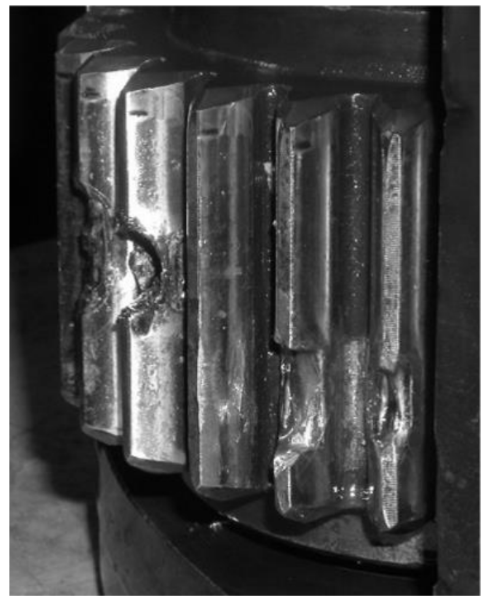
\includegraphics[scale=0.5]{images/uszkodzenie_kolko.png}
	\caption{Uszkodzony element maszyny górniczej}
	\label{uszkodzenie}
\end{figure}



\section{Opis problemu}
Uszkodzenia lokalne są uszkodzeniami występującymi w łożyskach i przekładniach maszyn górniczych. Ich powstawanie uzależnione jest od zmiennych warunków eksploatacyjnych \cite{adaptacyjne}. Uszkodzenie w początkowym stanie obniża sprawność maszyny a ostatecznie może doprowadzić do jej unieruchomienia. Jest to szczególnie problematyczne ponieważ kopalnia dysponuje często jedną lub dwiema takimi maszynami, dodatkowo każda z nich pracuje wyłącznie na swoim stanowisku, nie są one przemieszczane.
 Detekcja uszkodzenia we wstępnym stadium rozwoju jest ważnym zagadnieniem ponieważ pozwala z wyprzedzeniem określić moment konserwacji urządzenia. W detekcji uszkodzeń najczęściej wykorzystuje się diagnostykę wibroakustyczną. Przykład badania maszyny tą techniką zaprezentowano na ilustracji \ref{sensory}. Metoda polega na umieszczeniu sensora na obudowie urządzenia, następnie następuje pomiar drgań. Otrzymany sygnał zawiera pewien zakres informacji na podstawie których możemy wnioskować o zaistnieniu uszkodzenia w urządzeniu. W przypadku opisywanych uszkodzeń okazuje się że ich obecność objawia się poprzez cykliczne impulsy w sygnale.
% Sygnał z pulsacjami i bez pulsacji
\begin{figure}[ht]

\centering
                     
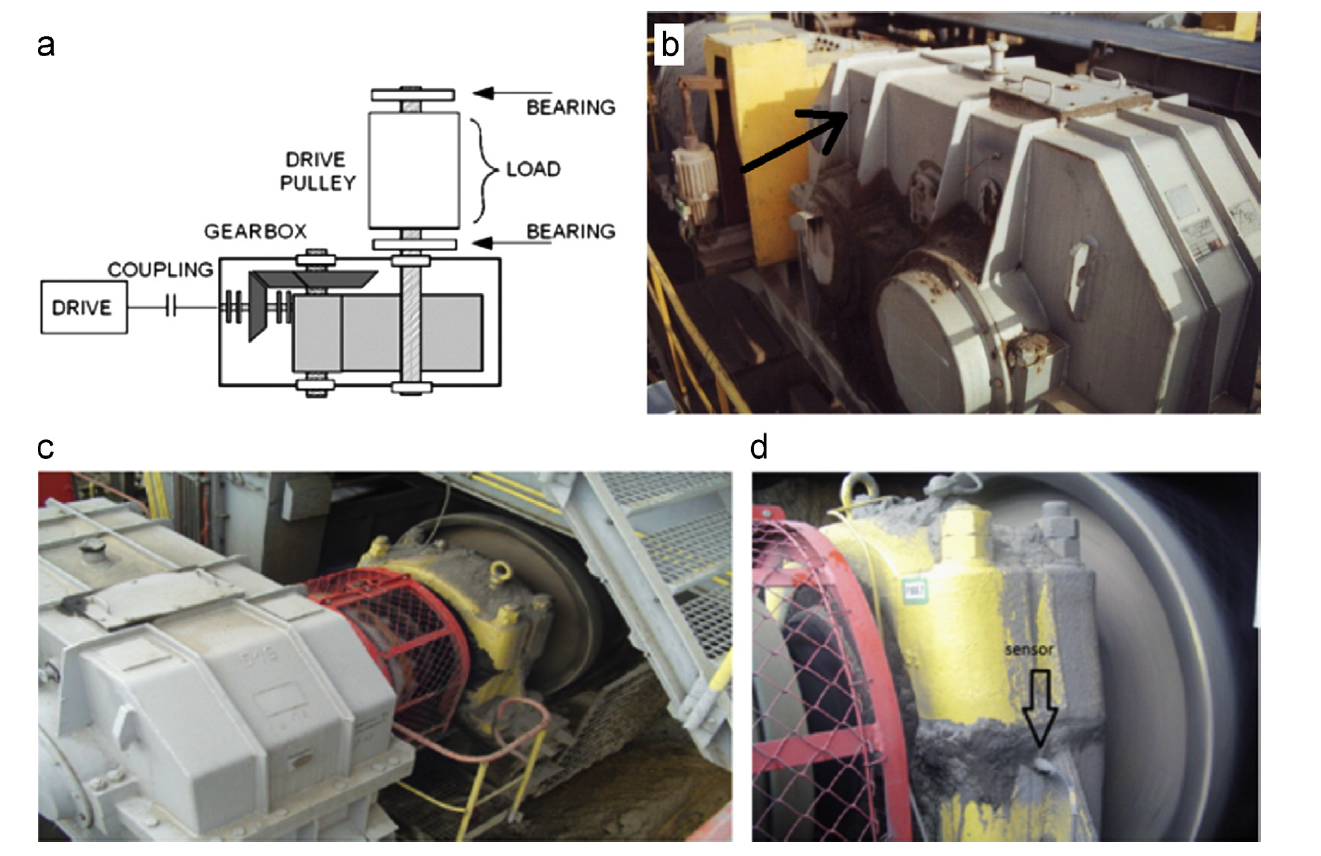
\includegraphics[scale=0.5]{images/sensors.png}
\caption{Schemat badanej maszyny ze wskazaniem miejsca lokalizacji sensorów diagnostycznych}
\label{sensory}
\end{figure}
Jednak w zależności od stopnia uszkodzenia pulsacje mogą mieć różne amplitudy, w przypadku wczesnego stadium rozwoju uszkodzenia najczęściej nie wystają one ponad poziom szumu. Przykłady sygnałów diagnostycznych przedstawione zostały na ilustracji~\ref{sygnal}.
Można zatem stwierdzić że detekcja uszkodzenia, z punktu widzenia matematyki, sprowadza się do wykrycia cyklicznych impulsów. 
\begin{figure}[ht]
	\centering
	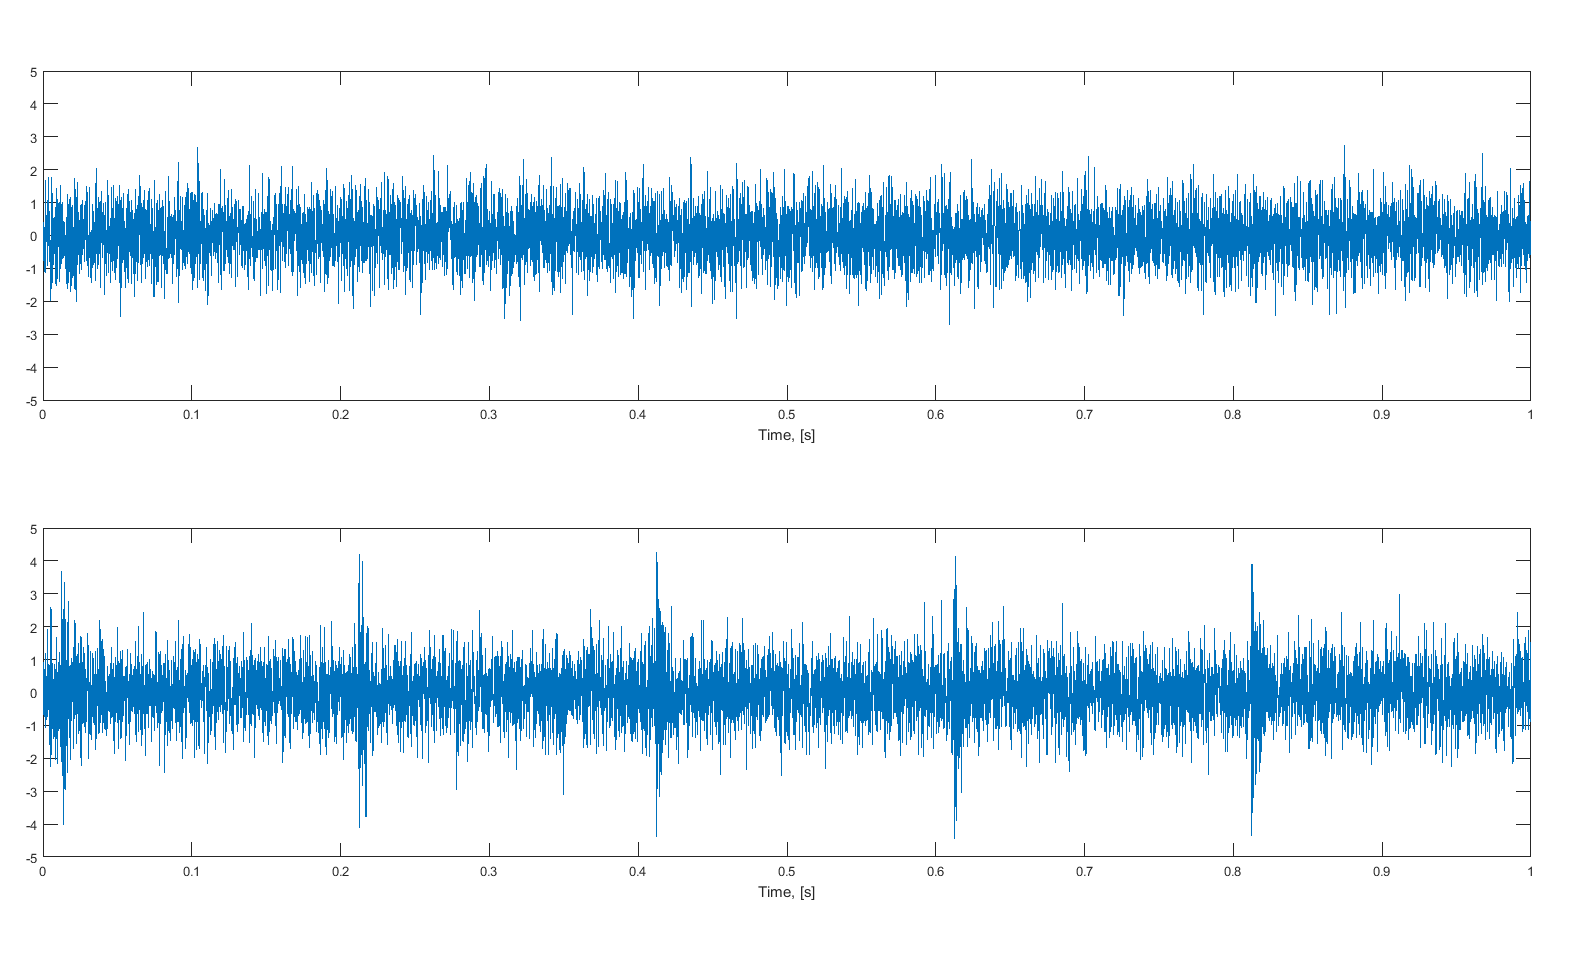
\includegraphics[scale=0.35]{images/zdrowy_pulsacja.png}
	\caption{Przykładowy sygnał diagnostyczny dla maszyny sprawnej (górny) oraz uszkodzonej (dolny)}
	\label{sygnal}
\end{figure}


%wykrywanie uszkodzeń lokalnych jest jednym z \cite{Zimroz01}
%Uszkodzenia lokalne powstające w przekładniach kół czerpakowych maszyn górniczych, są to na %przykład ubytki, pęknięcia, wykruszone zęby.  Najskutecznejszą obecnie metodą pozyskania sygnału %jest diagnostyka wibroakustyczna, okazuje się że uszkodzenia takie objawiają się cyklicznymi %pulsacjami w sygnale. Amplituda pulsacji zależy od stopnia uszkodzenia. Z punktu widzenia %matematyki detekcja takiego uszkodzenia polega na wykryciu, zazwyczaj niewidocznych na pierwszy %rzut oka, pulsacji w sygnale diagnostycznym. 

\section{State of the art}
Analiza sygnałów diagnostycznych pochodzących z urządzeń mechanicznych jest szeroko badanym zagadnieniem inżynierskim. W tym celu wykorzystuje się szereg technik a dzięki postępującym pracom zakres dostępnych narzędzi stale się powiększa. Wiedząc, że uszkodzenie objawia się modulacjami częstotliwościowymi i amplitudowymi. Rzeczą oczywistą staje się wykorzystanie narzędzi znanych z analizy sygnałów.
Interesującą techniką jest zautomatyzowane wyznaczanie pasma informacyjnego, zawierającego informacje o uszkodzeniu, z zastosowaniem filtrowania falkowego \cite{linandzuo}. 

Podejście zaproponowane przez Antoni \cite{antoni} polega na obliczeniu kurtozy dla poszczególnych częstotliwości wziętych ze spektrogramu. Pozwala to na użycie ich w dalszej kolejności do wyznaczenia momentów wysokiej zmienności i ich lokalizacji w dziedzinie częstotliwości. Rozwinięciem tego podejścia jest wykorzystanie diadycznej(??) dekompozycji sygnału, również używając kurtozy do wyznaczenia pasma częstotliwości. Podejście to nazwane kurtogramem również zostało rozszerzone przez kolejnych naukowców.???\cite{antoni2}

Urban \cite{urban} wykorzystuje rozkład intensywności modulacji do wyznaczania pasma informacyjnego. Podejście bazuje na założeniu istnienia nieliniowych zjawisk (???) (non-linear phenomena) powodowanych przez uszkodzenia lokalne. Dają się one modelować przez modulację amplitudową. 

Lub też użycie testu Andersona-Derlinga do obliczenia odległości od rozkładu normalnego, okazuje się że sygnał pochodzący z uszkodzonej maszyny jest daleki od takiego rozkładu. \cite{wylomanska} 
%prztumaczyc dokument ze strony wylomanskiej 
%{\Huge tutaj jakies odleglosci od rozkladu normalnego, spektrogramy itd}


\section{Sieci neuronowe}
Sieci neuronowe można zdefiniować jako struktury matematyczne realizujące obliczenia lub przetwarzające sygnały poprzez rzędy elementów zwanych sztucznymi neuronami.
Obecnie sieci neuronowe są jedną z prężnie rozwijających się technologii nauczania maszynowego i szeroko wykorzystywane w pracach nad sztuczną inteligencją.
Prężny rozwój dziedziny zapoczątkowało wynalezienie sztucznego perceptronu w 1957r. Był to model sztucznego neuronu pozwalającego na binarną klasyfikację liniowo separowalnych danych.

Wraz z upływem czasu pojawiają się kolejne modele neuronów i rodzaje sieci neuronowych. Dzisiaj problemy takie jak grupowanie danych, wykrywanie struktur, regresja nie stanowią dla sieci żadnego problemu. Potrafią one o wiele więcej. Wraz ze wzrostem mocy obliczeniowej komputerów oraz możliwości dokonywania na procesorach kart graficznych (GPU) możliwe stało się wielowarstwowych architektur a wielu węzłach, tak zwanych głębokich sieci neuronowych (\textit{ang. deep neural networks}). Te skomplikowane struktury potrafią o wiele więcej, a każdego dnia pojawia się więcej pomysłów na ich zastosowanie. 

Głębokie architektury sieci konwolucyjnych bez problemu radzą sobie z przetwarzaniem obrazów. Wykrywanie obiektów w czasie rzeczywistym \cite{ren2015faster}, rozpoznawanie twarzy \cite{lin1997face} czy prowadzenie pojazdu \cite{bojarski2016end} przez komputer nie wydaje się być dzisiaj niczym zaskakującym. Sieci takie pomagają również wykrywać zmiany nowotworowe \cite{nnnature} na podstawie zdjęć lub opisywać fotografie \cite{xu2015show}.

Co zaskakujące, sieci neuronowe pozwalają na coraz bardziej naturalną, z ludzkiego punktu widzenia, komunikację z maszynami. Dziedzina nazywana przetwarzaniem języka naturalnego (\textit{ang. natural language processing}) zajmuje się opracowaniem metod pozwalającym rozumieć maszynom nasz język \cite{nnspeech}. Rezultaty są zaskakujące, a możliwości obiecujące. W dobie tak zwanych asystentów nie jest już niczym dziwnym mówienie do maszyny, oglądanie wirtualnych prezenterów w telewizji. W przetwarzaniu języka zaskakująco skuteczne są tak zwane sieci rekurencyjne z pamięcią \cite{tai2015improved}.  Wnioskowanie kolejnego słowa w zdaniu jest ich ciekawym zastosowaniem. Dzięki nim smartfony potrafią przewidywać zakończenie zdania \cite{nngboard}, przygotować automatyczną odpowiedź, czy też napisać cały artykuł.

Wiedząc o tak zaawansowanych zastosowaniach i mając dowód skuteczności sieci neuronowych przeprowadzono eksperyment mający na celu zbadanie ich skuteczności w problemie wykrywania uszkodzeń lokalnych w sygnałach diagnostycznych pochodzących z maszyn górniczych. Dalsza część pracy opisuje wykorzystane metody, proces dochodzenia do rozwiązania oraz zastosowanie opracowanego modelu w systemie potrafiącym monitorować stan maszyny w czasie rzeczywistym.

\chapter{Metodologia}
Zakres wykonanej pracy obejmuje poszukiwanie optymalnego rozwiązania dla postawionego problemu. Na ten problem składają się wybór i przygotowanie danych uczących model oraz zaprojektowanie skutecznego modelu. 
W kolejnych krokach opisano narzędzia i techniki wykorzystane w tym celu. Ponieważ sieci neuronowe wymagają znaczącej ilości danych, a~ich zdobycie w przypadku zaawansowanych maszyn górniczych jest problematyczne, pracę należało zacząć od stworzenia sytemu symulowania sygnałów o zbliżonych cechach oraz wygenerowania zbioru danych (\textit{ang. dataset}). Następnie poruszony zostanie temat tak zwanej ekstrakcji cech, wstępnej obróbki danych w celu stworzenia najlepiej opisujących je cech. Finalnie możliwe jest przystąpienie do projektowania, trenowania i testowania sieci w celu stworzenia możliwie skutecznego modelu.
%\chapter{Sygnał diagnostyczny - symulowanie, wstępne przetwarzanie} 
\section{Symulowanie sygnału diagnostycznego}
\section{Wstępne przetwarzanie danych}
Przed przystąpieniem do uczenia sieci neuronowej niezbędne jest przygotowanie zestawu danych uczących. W dalszej pracy przetestowano dwa podejścia, jedno z użyciem surowego sygnału, drugie polegające na przygotowaniu statystyk opisujących sygnał. Zadanie polega na wykryciu pulsacji w sygnale diagnostycznym dlatego wybór statystyk opisujących sygnał musi odpowiadać postawionemu zadaniu. Dla opisania zmienności sygnału posłużą następujące estymatory:
\begin{itemize}
	\item Wartość maksymalna
	\item Wartość minimalna
	\item Wariancja
	\begin{equation}
	Var (X) = \frac{1}{n-1} \sum_{i=0}^{n} \left(x_{i} - \mu\right)^{2}
	\end{equation}
	\item Kurtoza
	\begin{equation}
	Kurt (X) = \frac{\frac{1}{n} \sum_{i=0}^{n}\left(x_{i} - \mu\right)^{4}}{\sigma^{4}} - 3
	\end{equation}
	\item Skośność
	\begin{equation}
	Skew (X) = 3 \frac{\mu - m}{\sigma}
	\end{equation}
\end{itemize}



\section{Zastosowanie sieci neuronowych}

Sieci neuronowe są strukturami realizującymi przetwarzanie danych poprzez rzędy elementów. Siecią użytą w pracy jest tak zwany perceptron wielowarstwowy. Jego bazowym elementem jest perceptron zaprezentowany poniżej. Składa się on z wejść wraz z wagami, funkcją sumującą oraz funkcją aktywacji. W przypadku użycia funkcji kroku perceptron pozwala na binarną klasyfikację liniowo separowalnych danych. 
\begin{figure}[ht]
	\centering
	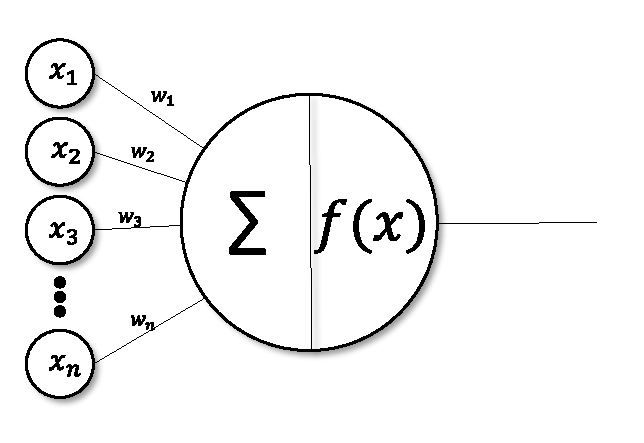
\includegraphics[width=10cm]{images/perceptron_c.pdf}
	\caption{Perceptron}
	\label{perceptron}
\end{figure}
W trakcie dalszych badań odkryto że połączenie wielu perceptronów pozwala na stworzenie struktury skutecznej nie tylko dla liniowo separowalnych danych. Tak powstał perceptron wielowarstwowy, popularna sieć neuronowa skuteczna w wielu zastosowaniach. Wyzwaniem jest wyznaczenie wag dla poszczególnych wejść. Najczęściej to zadanie jest realizowane poprzez algorytm wstecznej propagacji polegający na obliczaniu błędu na wyjściu z sieci a następnie przekazywaniu go wstecz tak aby poszczególne warstwy mogły zmodyfikować swoje wagi. 
\begin{figure}[ht]
	\centering
	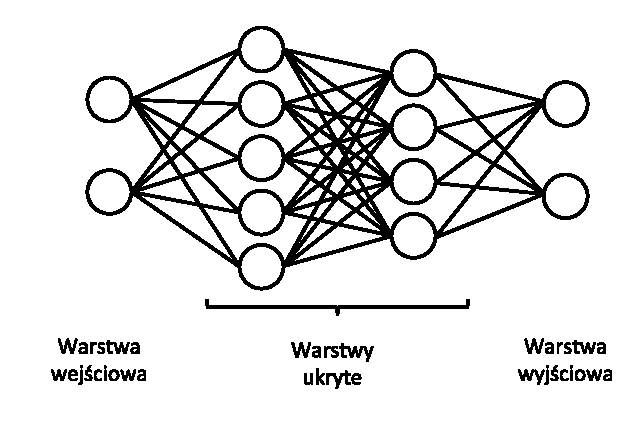
\includegraphics[width=10cm]{images/siec_c.pdf}
	\caption{Perceptron wielowarstwowy}
	\label{mlp}
\end{figure}

Testowanie skuteczności sieci odbywać się będzie przy pomocy techniki nazywanej walidacją krzyżową. Polega ona na podziale całości danych na części a następnie wybierane kolejno jednej z nich jako zbioru testowego, używając reszty danych do nauczenia sieci. Zbierając wyniki dla wykonanych prób możliwe jest określenie jakości rozwiązania. 
\begin{figure}[ht]
	\centering
	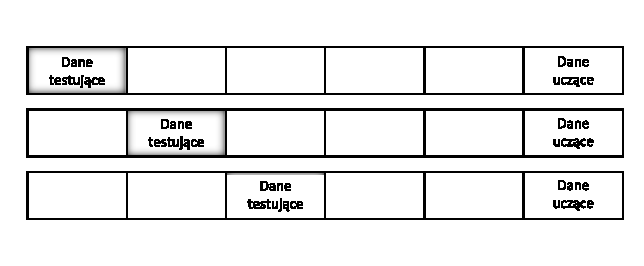
\includegraphics[width=10cm]{images/walidacja_c.pdf}
	\caption{Walidacja krzyżowa}
	\label{cross-validation}
\end{figure}

\section{Trening sieci neuronowej}
tutaj schemat kompletnego działąnia z podsumowaniem tego co bylo wczesniej i opisem jak dziala
Rysunek \ref{proces-caly} przedstawia schemat działania
\begin{figure}[ht]
	\centering
	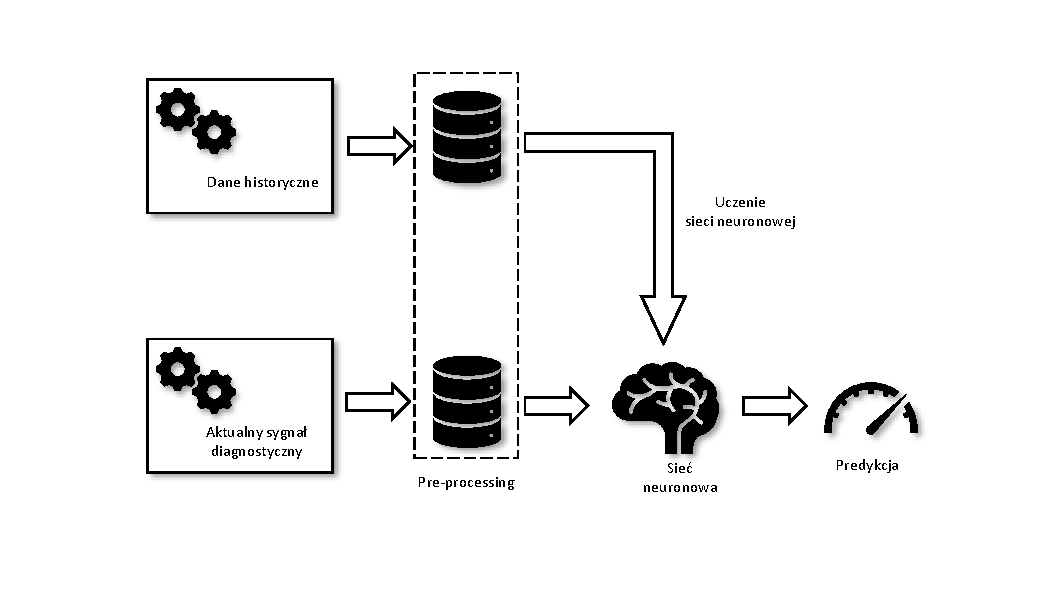
\includegraphics[scale=0.7]{images/total_proc.pdf}
	\caption{Schemat przebiegu pracy systemu wykrywania uszkodzenia}
	\label{proces-caly}
\end{figure}


\section{System klasyfikacji uszkodzeń}
Finalnym zadaniem jest stworzenie całości systemu monitorującego który dokonywałby predykcji na postawie wprowadzonego sygnału. 
\begin{figure}[ht]
	\centering
	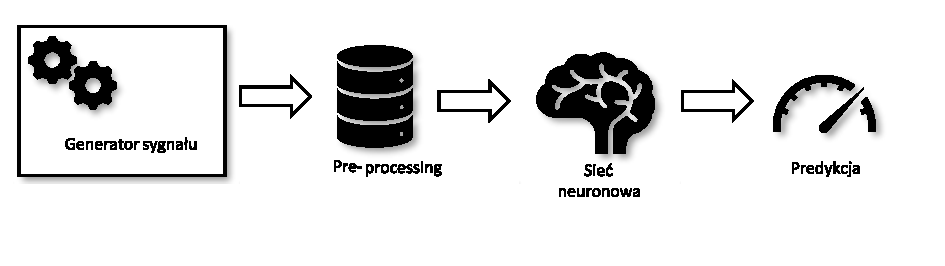
\includegraphics[scale=0.7]{images/workflow_c.pdf}
	\caption{Schemat przebiegu pracy systemu wykrywania uszkodzenia}
	\label{proces-koncowy}
\end{figure}

W dalszych rozdziałach opisany zostanie proces wykorzystania powyższych metod w celu opracowania optymalnego rozwiązania. Rozpoczynając od określenia metodyki projektowania i testowania sieci neuronowej poprzez trening i wybór najlepszego modelu. Ostatecznie zaprezentowane zostanie przykładowe zastosowanie opracowanego modelu w teoretycznym systemie monitorującym pracę maszyny górniczej. 



% opis dzialania sieci neuronowej jak sadze







%\chapter{Wyniki dla danych symulowanych}
\chapter{Projektowanie sieci neuronowej}
Skuteczność rozwiązania silnie zależy od użytej sieci. Projektowanie sieci polega na doborze tak zwanych hiperparametrów (\textit{ang. hyperparameters}). Zalicza się do nich między innymi:
\begin{itemize}
	\item Liczba warstw ukrytych
	\item Liczba neuronów w warstwach
	\item Algorytm nauczania oraz jego parametry
	\item Funkcje aktywacji w neuronach.
\end{itemize}

Nie istnieje skuteczna metoda doboru parametrów, przy zastosowaniu złożonych sieci badacze najczęściej polegają na swoim doświadczeniu oraz intuicji. Na potrzeby tego zadania przeprowadzono szereg eksperymentów mających na celu określić najskuteczniejszą sieć do wykonania postawionego zadania. \\

Żeby tego dokonać należy ustalić sposób pomiaru skuteczności danej sieci, w tym celu posłużono się macierzą pomyłek przedstawioną w tabeli \ref{tab:pomylki} oraz zdefiniowanymi przy jej pomocy miarami.

\begin{table}[ht]
	\caption{Macierz pomyłek}
	\begin{tabular}{lccc}
		& \multicolumn{1}{l}{}                    & \multicolumn{2}{c}{\textbf{klasa rzeczywista}}                                                                                                                                      \\ \cline{3-4} 
		& \multicolumn{1}{c|}{}                   & \multicolumn{1}{c|}{\textbf{pozytywna}}                                                  & \multicolumn{1}{c|}{\textbf{negatywna}}                                                  \\ \cline{2-4} 
		\multicolumn{1}{c|}{\multirow{2}{*}{\textbf{klasa predykowana}}} & \multicolumn{1}{c|}{\textbf{pozytywna}} & \multicolumn{1}{c|}{\begin{tabular}[c]{@{}c@{}}prawdziwie\\ pozytywna (TP)\end{tabular}} & \multicolumn{1}{c|}{\begin{tabular}[c]{@{}c@{}}fałszywie\\ pozytywna (FP)\end{tabular}}  \\ \cline{2-4} 
		\multicolumn{1}{c|}{}                                            & \multicolumn{1}{c|}{\textbf{negatywna}} & \multicolumn{1}{c|}{\begin{tabular}[c]{@{}c@{}}fałszywie\\ negatywna (FN)\end{tabular}}  & \multicolumn{1}{c|}{\begin{tabular}[c]{@{}c@{}}prawdziwie\\ negatywna (TN)\end{tabular}} \\ \cline{2-4} 
	\end{tabular}
\caption*{\textit{Źródło: opracowanie własne}}
\label{tab:pomylki} 
\end{table}

\begin{center}
	\begin{enumerate}
		\item Dokładność (\textit{ang. accuracy})
		\begin{equation}
		acc = \frac{TP + TN}{P + N}
		\end{equation}
		\item Czułość (\textit{ang. recall}) - odsetek prawdziwie pozytywnych
		\begin{equation}
		recall = \frac{TP}{TP + FN}
		\end{equation}
		\item Precyzja (\textit{ang. precision})
		\begin{equation}
		precision = \frac{TP}{TP + FP}
		\end{equation}
		\item F1 - średnia harmoniczna precyzji i czułości 
		\begin{equation}
		F1 = 2 \cdot \frac{precision \cdot recall}{precision + recall}
		\end{equation}
	\end{enumerate}
	
\end{center}

Badanie skuteczności sieci opiera się na metodyce walidacji krzyżowej czyli podziału zbioru danych na części a następnie użycie każdej z kolejno do testowania, reszta do uczenia <- to do metodyki


\section{Zależność od danych wejściowych}
Pierwszy eksperyment będzie postawą do decyzji o tym jakich danych należy użyć do uczenia sieci. Należy porównać jak uczy się sieć w zależności od danych wejściowych. Porównane zostaną dwa podejścia: użycie surowego sygnału oraz wstępnie przetworzonego. 

\begin{enumerate}
	\item Surowy sygnał podeście pierwsze
	\subitem dane wejściowe: 4096
	\subitem warstwy ukryte: 1000 - 500 - 200
	\subitem liczba wag: 
	
	\item Surowy sygnał podejście drugie
	\subitem dane wejściowe: 4096
	\subitem warstwy ukryte: 500 - 200
	\subitem liczba wag:
	
	\item Estymatory sygnału
	\subitem dane wejściowe: 8
	\subitem warstwy ukryte: 5 - 3 - 2
	\subitem liczba wag: mało
\end{enumerate}

Wyniki eksperymentu prezentują sie następująco.


\begin{figure}[ht]
	\centering
	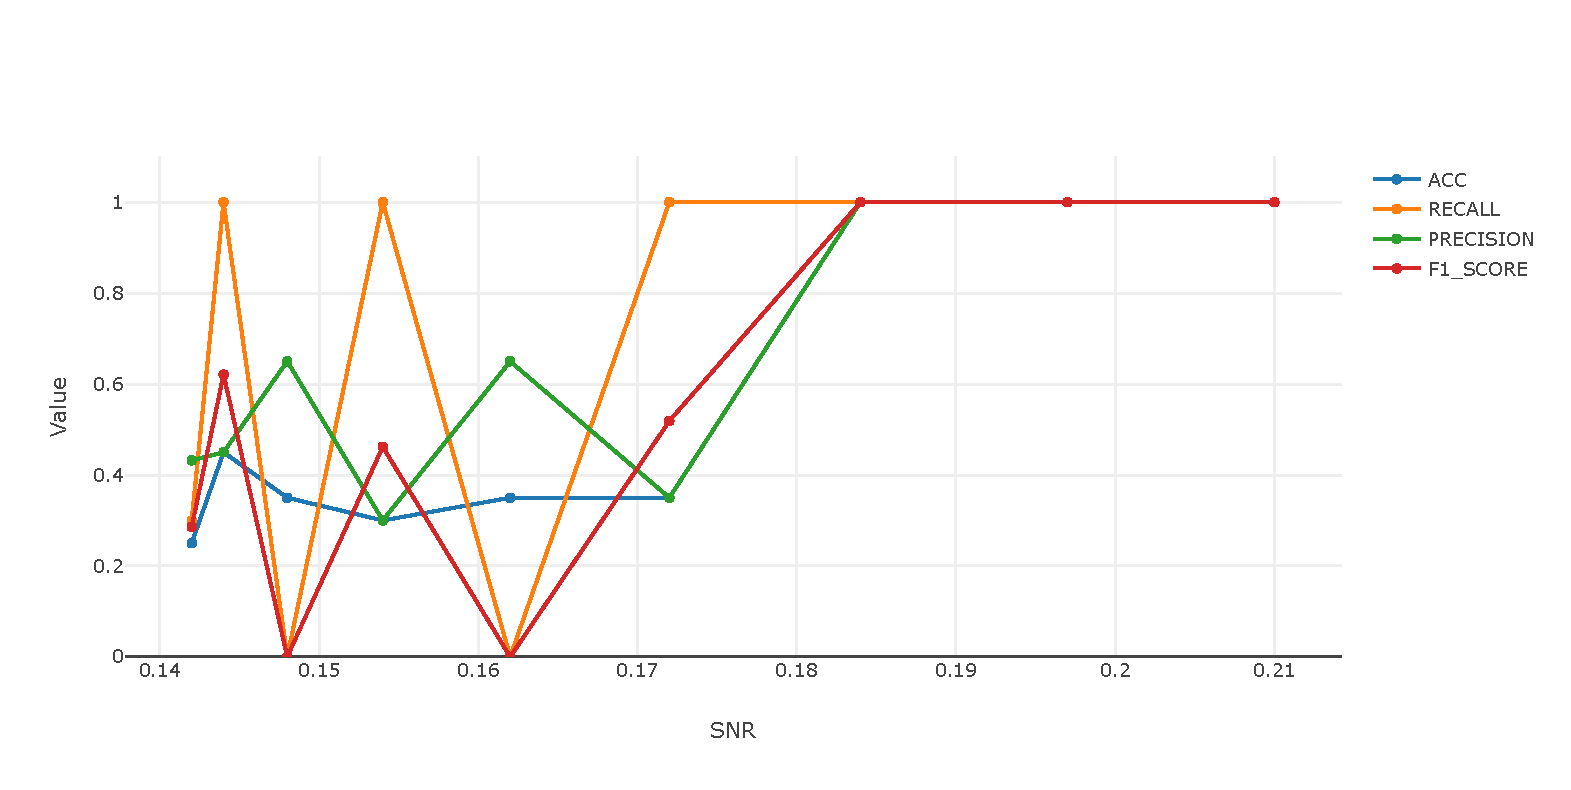
\includegraphics[width=14cm]{images/nn_full_1000_500_200.pdf}
	\caption{Wyniki surowego sygnału, architektura -1000-500-200-}
	\label{wynik-sur-1000-500-200}
\end{figure}

\begin{figure}[ht]
	\centering
	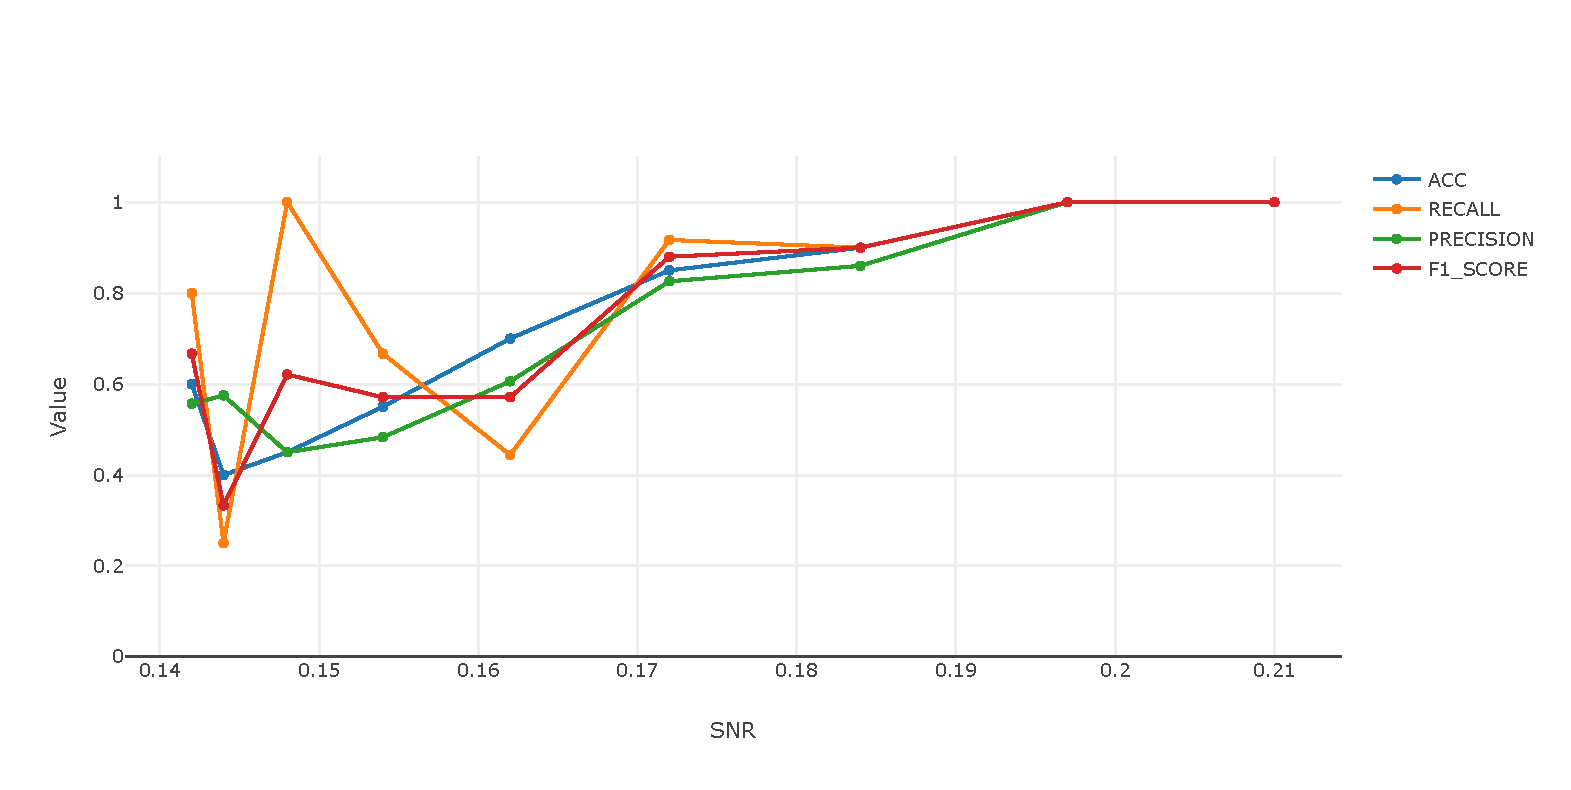
\includegraphics[width=14cm]{images/nn_full_signal_500_200.pdf}
	\caption{Wyniki dla surowego sygnału, architektura -500-200-}
	\label{wynik-sur-500-200}
\end{figure}

\begin{figure}[H]
	\centering
	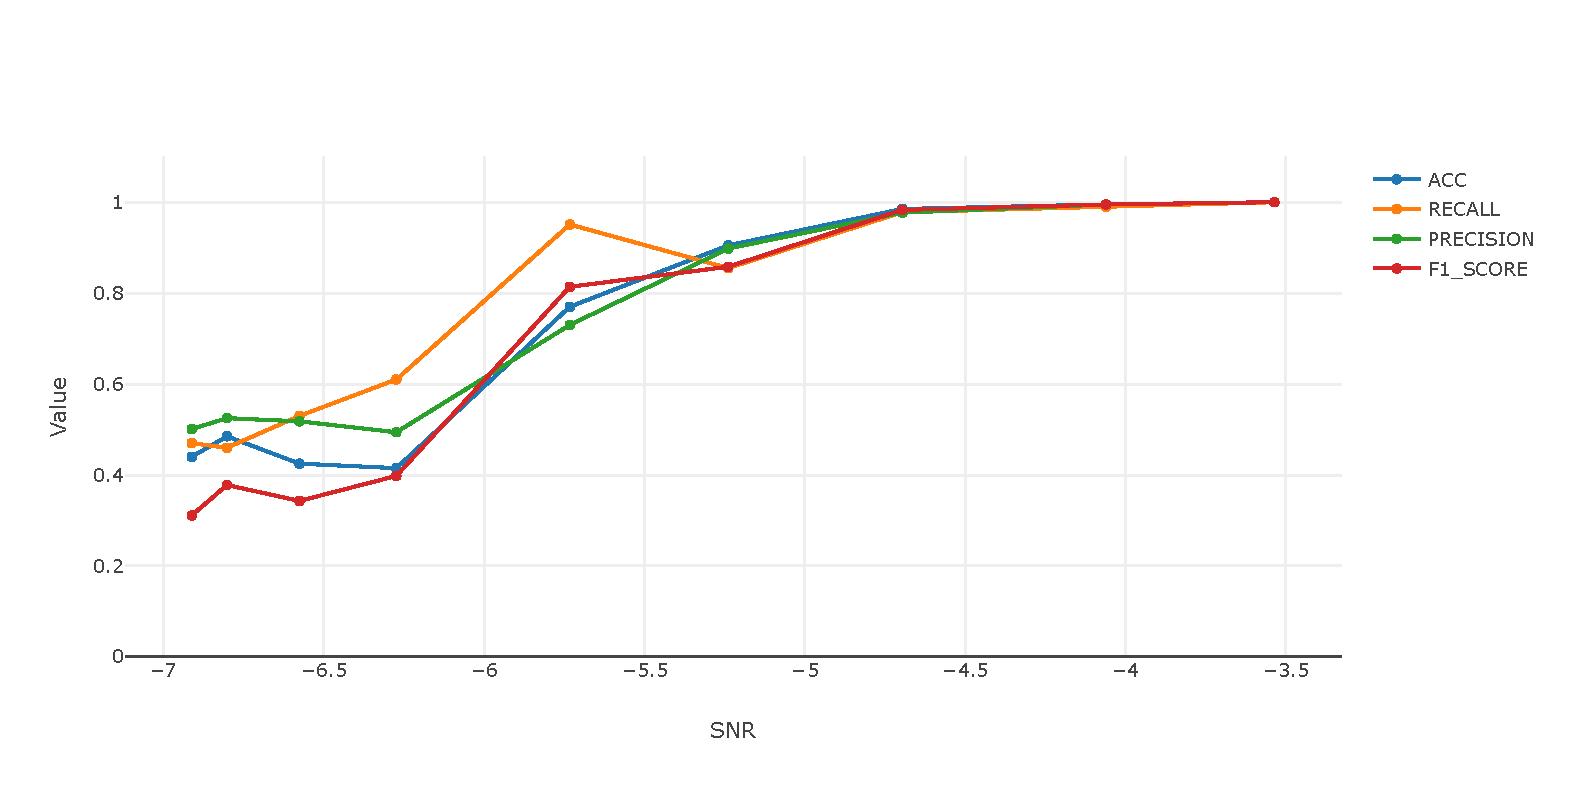
\includegraphics[width=14cm]{images/nn_small_532.pdf}
	\caption{Wyniki dla estymatorów, architektura -5-3-2-}
	\label{wynik-est-5-3-2}
\end{figure}

Zastosowanie surowego sygnału, niezależnie od architektury, daje bardzo chaotyczne wyniki sugerujące że proces nauczania nie przebiega prawidłowo a predykcja jest obarczona dużym błędem. Podejście z zastosowaniem surowego sygnału jest kosztowne obliczeniowo i mało efektywne dlatego należy je wykluczyć z dalszych rozważań. Z kolei zastosowanie estymatorów opisujących sygnał daje obiecujące wyniki pozwalające wnioskować o skutecznym uczeniu się sieci. W oparciu o zaproponowaną architekturę zostanie przeprowadzony kolejny eksperyment mający stwierdzić czy przy użyciu obecnych danych uczących można otrzymać lepsze wyniki.

\section{Zależność od architektury}
Po decyzji o użyciu estymatorów jako danych uczących należy przeprowadzić eksperyment mający na celu określenie najlepszej architektury sieci neuronowej. Ponieważ architektura zaproponowana w poprzednim eksperymencie dawała wyniki świadczące o poprawnie przebiegającym procesie uczenia zaproponowano różne jej wariancje. 
\begin{figure}[ht]
	\centering
	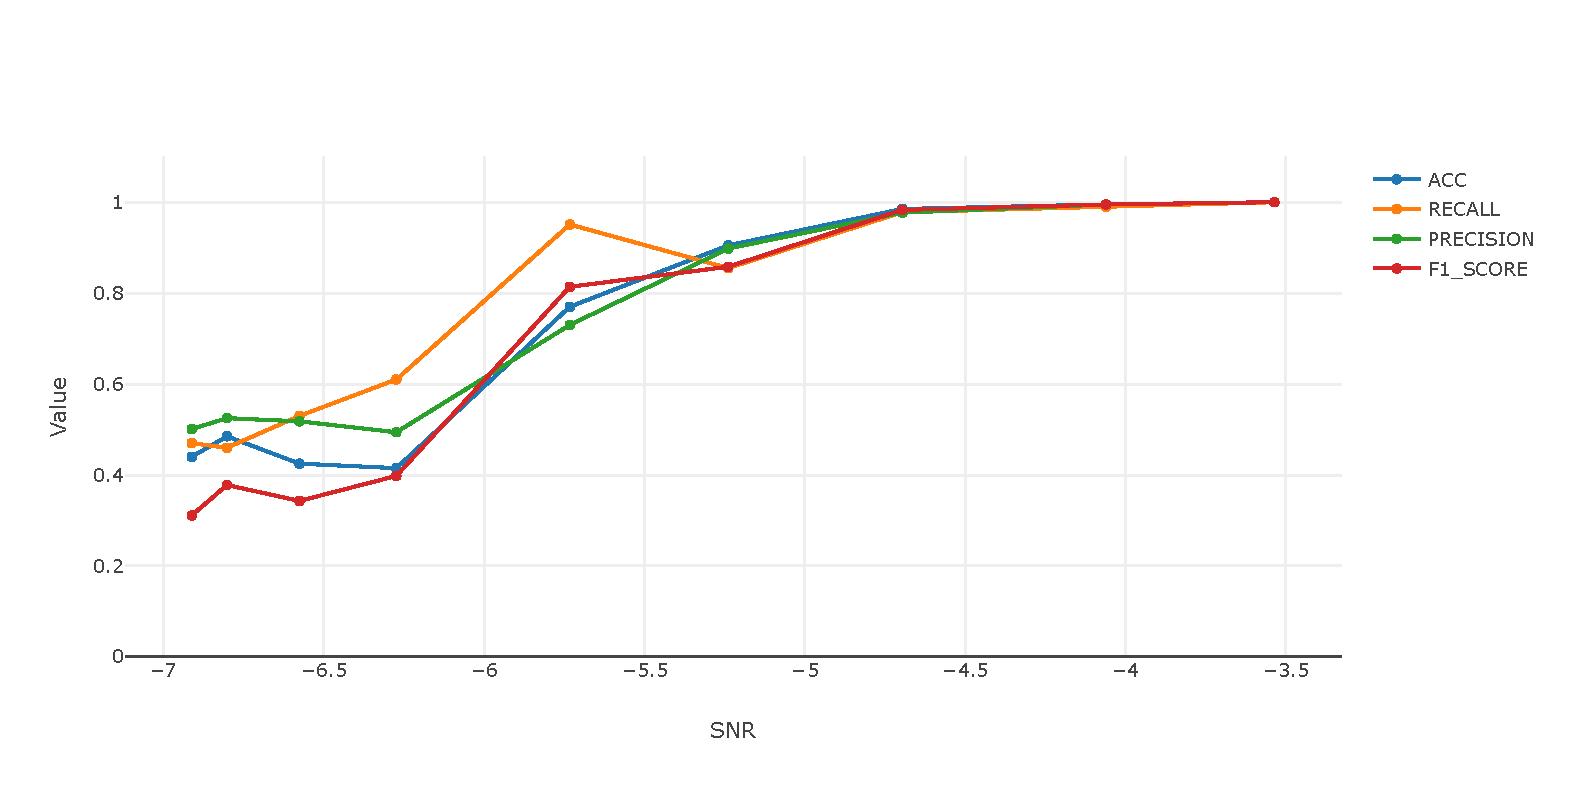
\includegraphics[width=14cm]{images/nn_small_532.pdf}
	\caption{Wyniki dla sieci o architekturze -5-3-2-}
	\label{wynik2-est-5-3-2}
\end{figure}
\begin{figure}[ht]
	\centering
	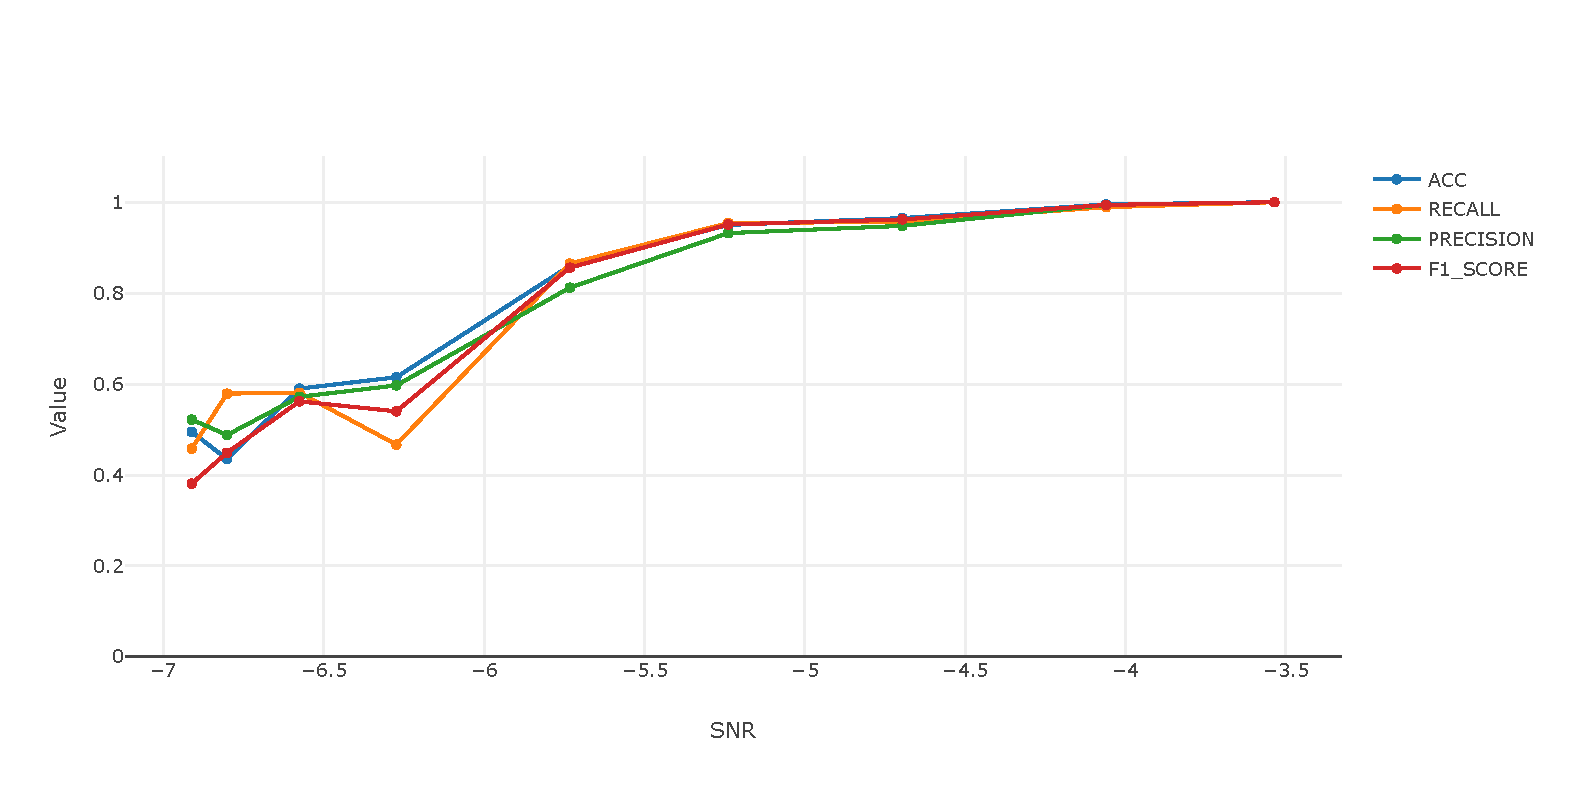
\includegraphics[width=14cm]{images/nn_small_85.pdf}
	\caption{Wyniki dla sieci o architekturze -8-5-}
	\label{wynik-est-8-5}
\end{figure}
\begin{figure}[ht]
	\centering
	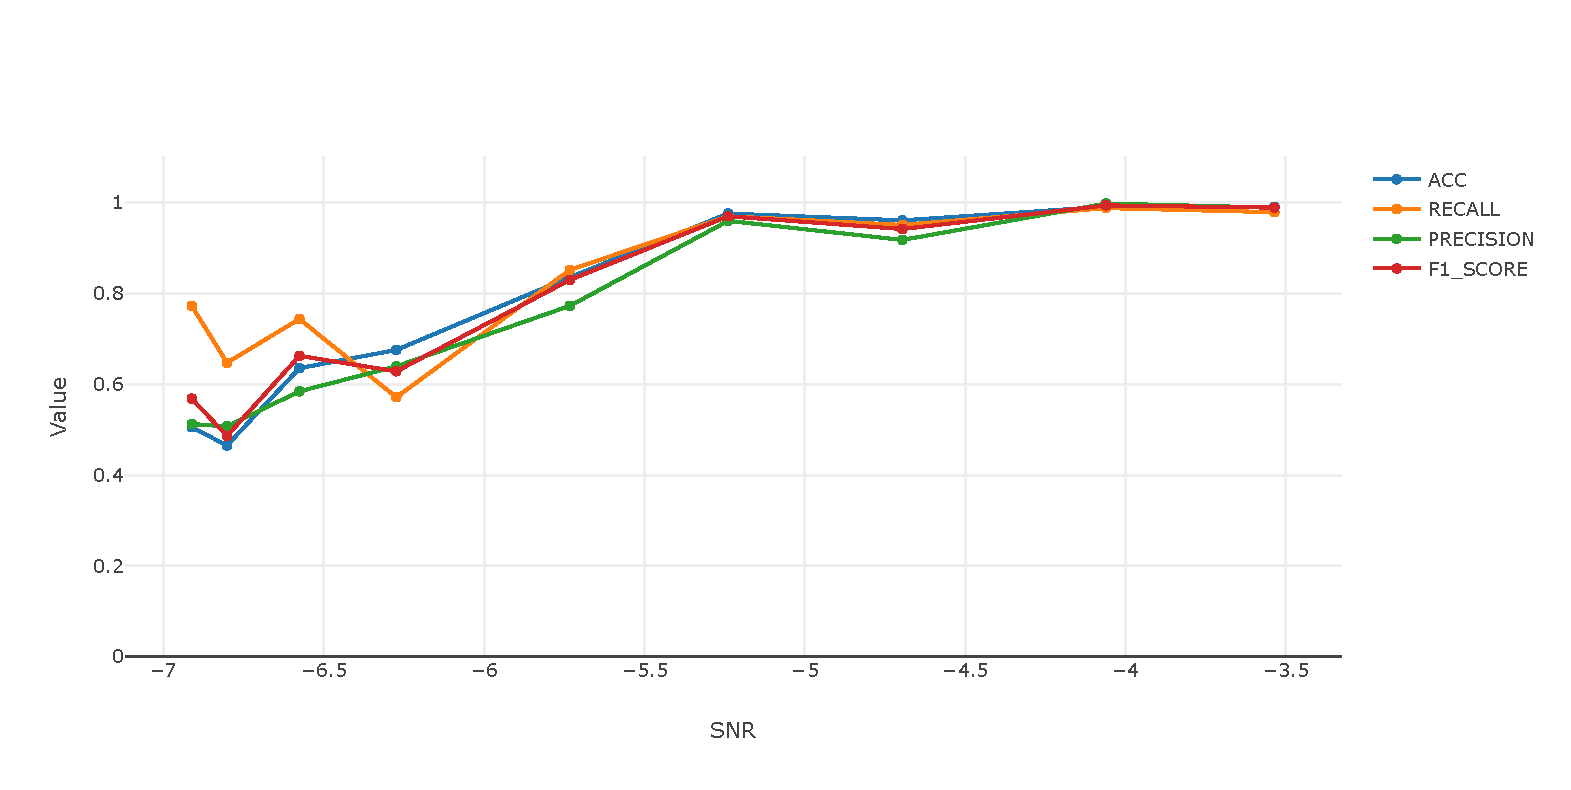
\includegraphics[width=14cm]{images/nn_small_2.pdf}
	\caption{Wyniki dla sieci o architekturze -2-}
	\label{wynik-est-2}
\end{figure}
\begin{figure}[ht]
	\centering
	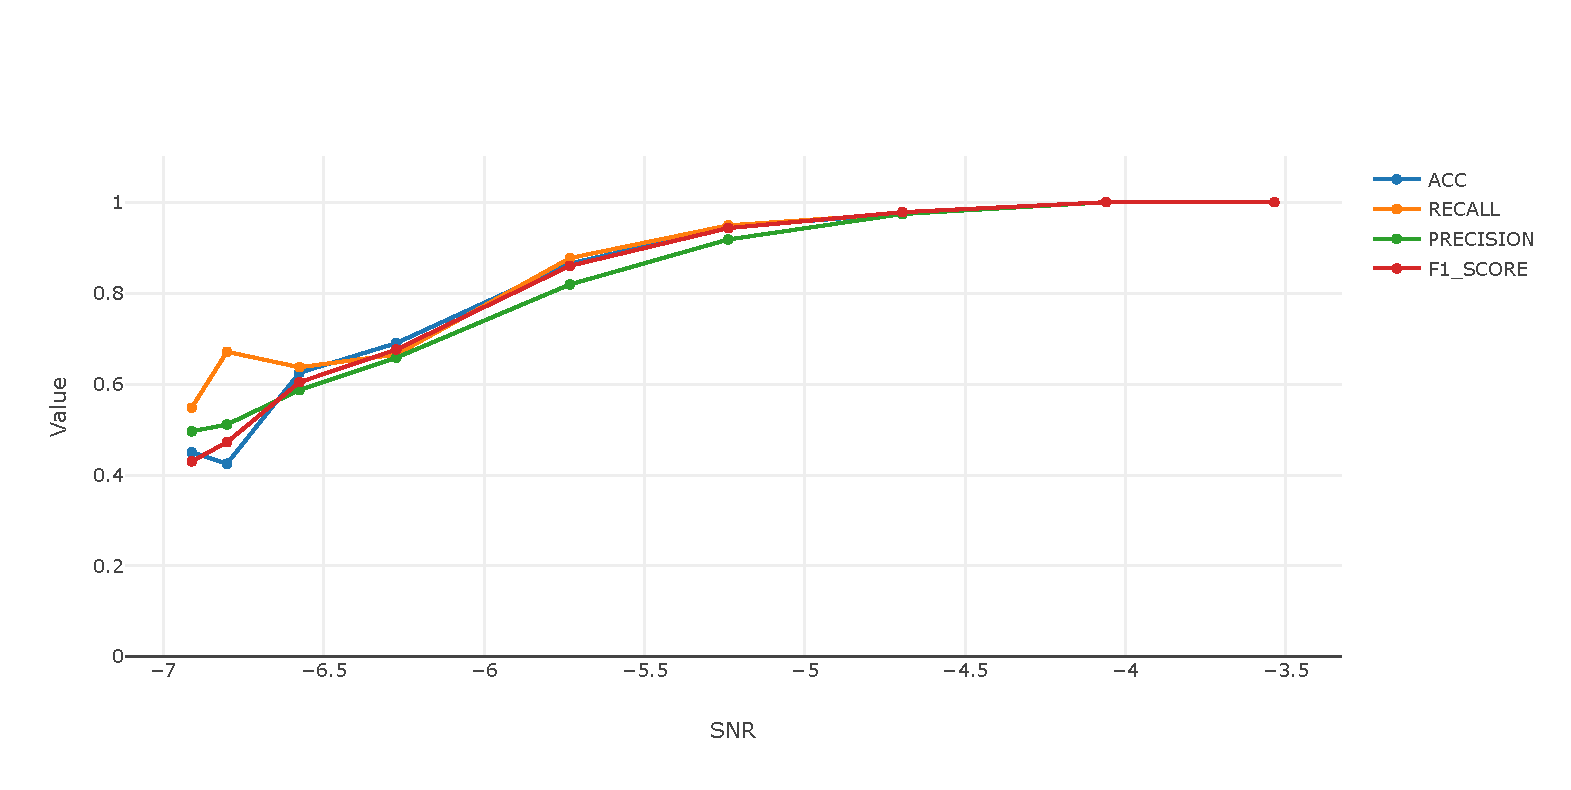
\includegraphics[width=14cm]{images/nn_small_5.pdf}
	\caption{Wyniki dla sieci o architekturze -5-}
	\label{wynik-est-5}
\end{figure}




%Nauczanie sieci 
%Z powodu zapotrzebowania na dużą ilosć danych w procesie uczenia sieci neuronowych dalsza praca opiera się na danych symulowanych. Program generujący sygnał pozwala na dobór szeregu parametrów takich jak częstotliwości, amplitudy, zaszumienie oraz siłę pulsacji.
%\subsection{Przygotowanie danych}
%Przed przystąpieniem do uczenia należało przygotować dane uczące, w tym przypadku jest to zestaw sygnałów bez pulsacji oraz sygnałów z różnymi pulsacjami, poniżej przedstawiono tabelkę szczegółowo opisującą przygotowany zbiór danych.
%\subsection{Surowy sygnał}
%Pierwszym eksperymentem było przetestowanie jak sieć poradzi sobie w przypadku surowych danych. Do nauczania użyto sygnału odpowiadającemu jednej sekundzie odczytu, co przy próbkowaniu na poziomie $x$ daje $w chuj$ próbek.
%\\ Tutaj jebniesz schemat sieci
%\\A tutaj tabelka z wniami 
%Eksperyment ten przeprowadzony był bardziej dla porównania niż z żeczywistej potrzeby, użycie surowego sygnału i takiej ilości próbek nie wydaje się był optymalnym rozwiązaniem za to jest kosztowne, dobrą praktyką w dziedzinie nauczania maszynowego jest wstępna obróbka danych i znalezienie sposobu na 

%\subsection{Estymatory}

%\chapter{Wnioski}


%\section{System monitorujący - przykładowe zastosowanie modelu}
\chapter{System monitorujący - przykładowe zastosowanie modelu}
%\chapter{Wnioski}
{\backmatter \chapter{Wnioski}}
\newpage




%{\backmatter \chapter{Wstęp}}
%We wstępie zapowiadamy, o czym będzie praca. Próbujemy zachęcić czytelnika do dalszej lektury, np. krótko informując, dlaczego wybraliśmy właśnie ten temat i co nas w nim zainteresowało.
%
%\chapter{Rozdział pierwszy}
%Tabela \ref{tab:przykladowa} przedstawia przykładową tabelę. Do tworzenia tabeli służą m.in. środowiska \texttt{tabular} oraz \texttt{table}. Istnieje możliwość numeracji dwustopniowej, gdzie pierwsza cyfra oznacza numer rozdziału, a druga – kolejny numer tabeli w tym rozdziale. Tytuł powinien znajdować się centralnie nad tabelą, $12$ pkt odstępu od tekstu zasadniczego nad i pod tabelą wraz z tytułem. Jeśli tabela jest cytowana – należy podać centralnie pod tabelą źródło jej pochodzenia, np. opracowanie własne, opracowano na podstawie danych z GUS.
%\begin{table}[ht]
%\caption{Podstawowa Tabela}
%\centering
%\begin{tabular}{ccc}
%\hline
%\hline                       
%Państwo & PKB (w milionach USD )& Stopa bezrobocia  \\  [0.5ex] 
%\hline 
%Stany Zjednoczone & 75 278 049 & 4,60\%  \\
%Chiny & 11 218 281 & 4,10\%   \\
%Japonia & 4 938 644 & 3,10\%  \\
%Niemcy & 3 466 639 & 6,00\%   \\
%Wielka Brytania & 2 629 188 & 4,60\%  \\ [1ex]  
%\hline 
%\end{tabular}
%\caption*{\textit{Źródło: opracowanie własne}}
%\label{tab:przykladowa} 
%\end{table}
%
%Do cytowania używamy komendy \texttt{cite}. W nawiasie klamrowym podajemy klucz, którego użyliśmy w pliku \emph{bibliografia.bib}. Przykład: \cite{einstein} lub \cite[chap. 2]{latexcompanion}.
%
%\section{Podrozdział pierwszy}
%
%\begin{table}[H]
%\caption{Podstawowa Tabela}
%\centering
%\begin{tabular}{ccc}
%\hline
%\hline                       
%Państwo & PKB (w milionach USD )& Stopa bezrobocia  \\  [0.5ex] 
%\hline 
%Stany Zjednoczone & 75 278 049 & 4,60\%  \\
%Chiny & 11 218 281 & 4,10\%   \\
%Japonia & 4 938 644 & 3,10\%  \\
%Niemcy & 3 466 639 & 6,00\%   \\
%Wielka Brytania & 2 629 188 & 4,60\%  \\ [1ex]  
%\hline 
%\end{tabular}
%\caption*{\textit{Źródło: opracowanie własne}}
%\label{tab:przykladowa2} 
%\end{table}
%
%\section{Podrozdział drugi}
%
%Rysunki do pracy dyplomowej należy wstawiać w sposób podobny do wstawiania tabel, z~zasadniczą różnicą polegającą na tym, że podpis powinno umieszczać się centralnie pod rysunkiem, a nie powyżej niego. Numeracja i sposób cytowania pozostają bez zmian, przy czym tabele i rysunki nie mają numeracji wspólnej, np. po Tabeli \ref{tab:przykladowa2} występuje Rysunek \ref{rys1} (o ile jest to pierwszy rysunek rozdziału pierwszego), a nie Rysunek $1.3$.
%
%\begin{figure}[ht]
%
%\centering
%                     
%
\includegraphics[scale=0.27]{logo_w13.jpg}
%\caption{Podstawowy Rysunek}\label{rys1}
%\end{figure}
%\label{rys:przykladowy} 
%
%
%\chapter{Definicje, lematy, twierdzenia, przykłady i wnioski}
%Definicje, lematy, twierdzenia, przykłady i wnioski piszemy w pracy tak:
%\begin{definition}[Martyngał]
%Tu piszemy treść definicji martyngału.
%\end{definition}
%\begin{lemma}[]% w nawiasie kwadratowym można napisać jego nazwę
%Tu piszemy treść lematu.
%\end{lemma}
%
%{\backmatter \chapter{Podsumowanie}}
%Podsumowanie w pracach matematycznych nie jest obligatoryjne. Warto jednak na zakończenie krótko napisać, co udało nam się zrobić w pracy, a czasem także o tym, czego nie udało się zrobić.
%
%{\backmatter \chapter{Dodatek}}
%Dodatek w pracach matematycznych również nie jest wymagany. Można w nim przedstawić np. jakiś dłuższy dowód, który z pewnych przyczyn pominęliśmy we właściwej części pracy lub (np. w przypadku prac statystycznych) umieścić dane, które analizowaliśmy.

%%%%%%%%%%%%%%%%%%%%%%%%%%%%%%%%%%%%%%%%%%%%%%%%%%%%%%%%%
% BIBLIOGRAFIA
% W tworzeniu bibliografii najlepiej korzystać z BibTex'a, 
% który jest częścią systemu Tex. W naszym przypadku funkcję 
% przechowalni literatury, do której się odwołujemy, pełni 
% plik bibliografia.bib. Nie musimy ręcznie dodawać nowych 
% pozycji do bibliografii. Możemy wejść np. na stronę 
% https://mathscinet.ams.org/mathscinet/index.html, 
% znaleźć odpowiednią pozycję, wybrać ją, a następnie zmienić 
% 'Select alternative format' na BibTeX, skopiować uzyskany 
% tekst, wkleić do pliku bibliografia.bib i skompilować. 
% Gotowe informacje do pliku bibliografia.bib można znaleźć 
% także na https://arxiv.org - gdy znajdziemy interesującą nas 
% pracę, szukamy 'References & Citations' i klikamy 'NASA ADS', 
% a potem 'Bibtex entry for this abstract' 
% i postępujemy tak jak wcześniej.
%%%%%%%%%%%%%%%%%%%%%%%%%%%%%%%%%%%%%%%%%%%%%%%%%%%%%%%%%
% w nawiasie klamrowym wpisujemy nazwę pliku z bibliografią w formacie .bib
\bibliography{bibliografia_backup} 
\bibliographystyle{bibliografia_styl}
\end{document}